\chapter{TSN测试平台的目标}
本平台利用ADI公司的TSN评估套件,测试在IEEE 802.1AS和802.1 Qbv标准框架下的数据传输方案,并开发出相匹配的测试软件。

\chapter{TSN评估板的简介}

\section{TSN评估板的构造组成}

%图2-1
\begin{figure}[h]
    \centering
    \label{structure1}
    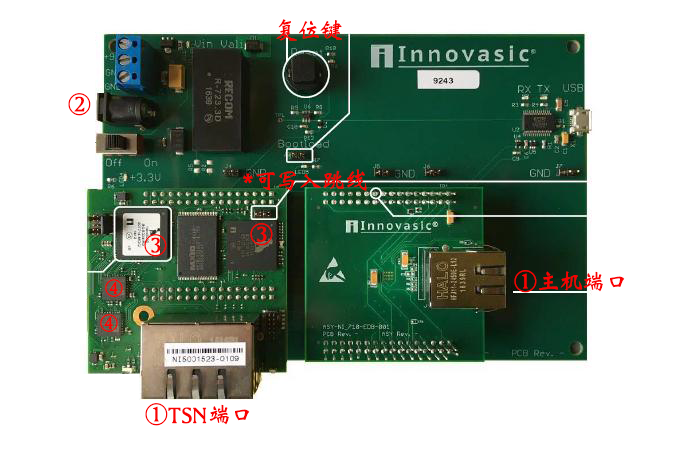
\includegraphics[width=0.6\textwidth]{pic/composition.png}
    \caption{}
\end{figure}

\begin{itemize}
    \item \textcircled{1} \textbf{评估板端口:}评估板总共有三个端口,位于其中之一是主机端口,位于印刷电路板(PCB)较窄的一侧,必须连接现有以太网设备。器件的标准以太网流量转发到交换机TSN端口(位于PCB较宽的一侧)。这种转发必须在配置任何TSN特性之前正常工作;
    \item \textcircled{2} \textbf{电源端口:}电路板设计支持9 V至24 V直流电压,本平台采用12V-1A的电源适配器,为电路板提供电源;
    \item \textcircled{3} \textbf{FIDO REM交换机:}它是整个TSN评估板套件的核心,是标准以太网设备连接到TSN网络的关键部件;
    \item \textcircled{4} \textbf{KSZ8061MNGW:}该芯片支持10BASE/100BASE-TX,它是一个用于通过非屏蔽双绞线(UTP)传输和接收数据的以太网物理层收发器;
    \item \textbf{可写入跳线:}修改MAC地址时,必须将其短路。
\end{itemize}

\section{TSN评估板的网络连接}

%图2-2
\begin{figure}[h]
    \centering
    \label{structure2}
    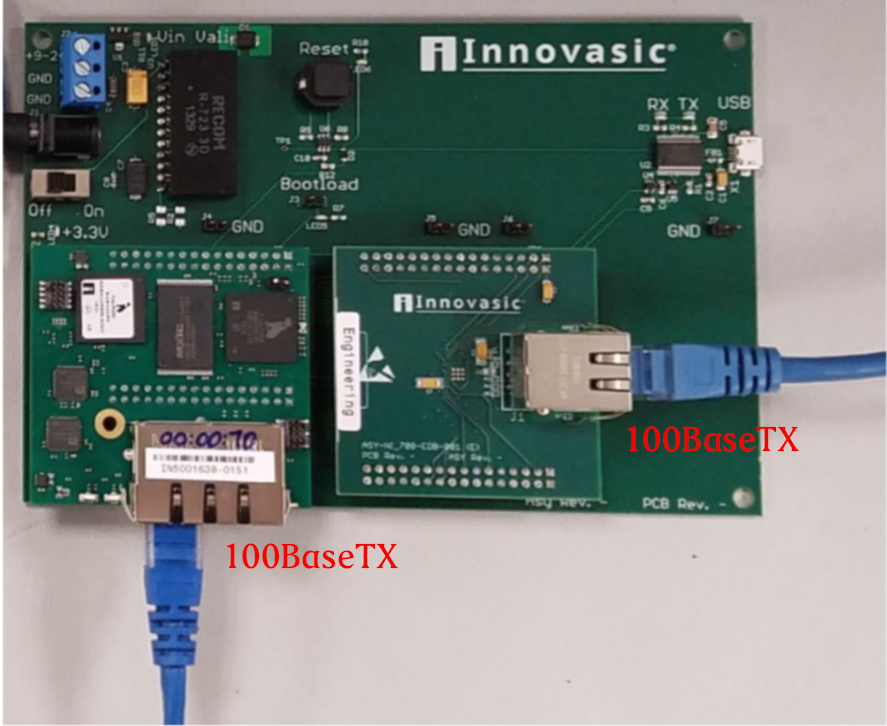
\includegraphics[width=0.5\textwidth]{pic/connection.png}
    \caption{}
\end{figure}

\begin{itemize}
	\item \textbf{支持协议:} EtherNet/IP,PROFINET RT,ModbusTCP和BACnet IP等;
	\item \textbf{不支持协议:} PROFINET IRT,EtherCAT,SERCOS 和 POWERLINK;
	\item \textbf{网络连接:} 三个端口均是100BaseTX;100表示传输速率为100Mbit/s,base表示采用基带传输,T表示传输介质为双绞线,当为F时,代表为光纤;X为统一传输速率下的不同标准,TX表示传输介质为2对高质量的双绞线。
\end{itemize}

\section{TSN评估板的内部结构图}
\begin{figure}[h]
	\centering
	\label{structure3}
	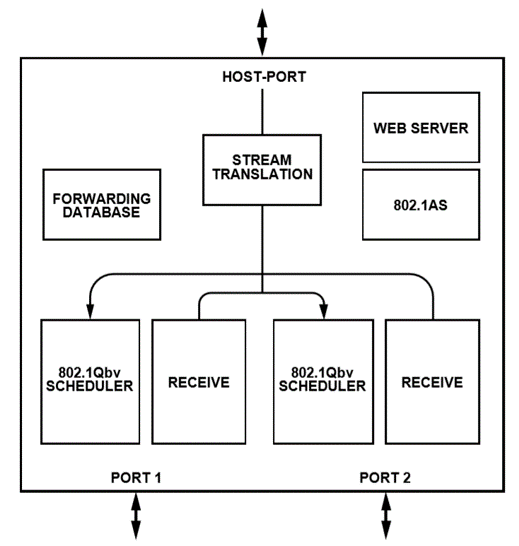
\includegraphics[width=0.5\textwidth]{pic/instructure.png}
	\caption{}
\end{figure}

\chapter{TSN平台搭建方案}

\section{线性拓扑结构}

\begin{enumerate}
	\item \textbf{结构组成}:摄像头、电脑以及TSN评估板;端口a代表TSN端口,端口b代表主机端口;
	\item \textbf{结构介绍}:最左端TSN端口链接PC,最右端TSN端口链接摄像头;中间TSN评估板构成TSN网络,可以连接支持TSN的设备;主机端口可以链接支持标准以太网设备。
\end{enumerate}

\begin{figure}[h]
    \centering
    \label{structure4}
    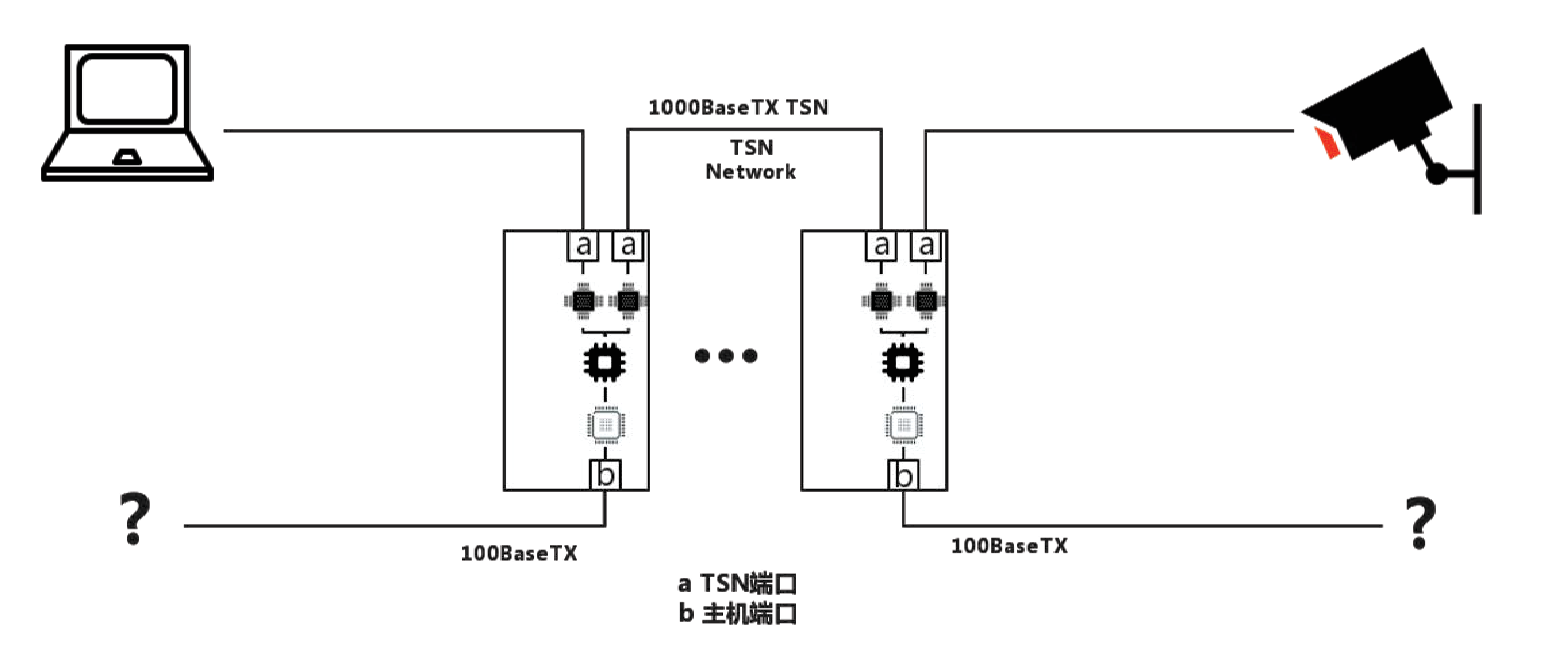
\includegraphics[width=0.8\textwidth]{pic/netstructure.eps}
    \setlength{\abovecaptionskip}{1pt}
\setlength{\belowcaptionskip}{1pt}
    \caption{}
\end{figure}

\section{TSN网络配置}

\subsection{TSN网关设置}

\begin{itemize}
    \item \textbf{TSN评估板套件MAC}和\textbf{IP地址}的配置:TSN评估板套件都配有唯一媒体访问控制(MAC)地址和唯一IP地址,但是每个TSN评估板的初始MAC地址(12:34:56:78:9A:BC)和IP地址(192.168.1.1)都一样,因此需要我们自行修改它们的MAC地址和IP地址;
    \item \textbf{子网掩码}的配置:默认为255.255.255.0;
    \item \textbf{主机端口MAC地址}的配置:在配置界面上的\textbf{Client MAC文本框}中输入\textbf{主机端口链接设备的MAC地址},实现数据链路层的互联互通。
\end{itemize}

\begin{quote}
\kaishu
\textcolor{red}{注意:} 
\begin{enumerate}
\item 在修改上述MAC地址和IP地址时,首先需要\textcolor{red}{将可写入跳线短路},重新上电之后,MAC地址和IP地址才能发生改变!
\item 通过\textcolor{red}{主机端口无法访问}配置网站,必须将PC连接到一个TSN端口才能进入配置网站。虽然主机端口连接PC时,不能访问该TSN评估板的配置网站,但是它可以访问另外\textcolor{red}{两个TSN评估板的配置网站}。原因在于该PC其实是连接到另外两个TSN评估板的TSN端口上。
\end{enumerate}
\end{quote}

\subsection{时间同步配置}

\begin{itemize}
	\item \textbf{时钟同步状态灯}:完成上述设置之后,802.1AS时间同步即可运行:其中一个电路板承担Grandmaster clock的角色,标志是其802.1AS\textbf{状态LED变红};在同步从设备上,当时钟同步已建立时,802.1\textbf{状态LED变绿}。
	\item \textbf{查看AS状态}:通过TSN评估板的配置界面可以查看评估板的状态,若TSN评估板是Grandmaster,Sync State显示Grandmaster;若TSN评估板不是宗时钟,如果与宗时钟同步,显示Synchronized,否则显示Unsynchronized。
	\item \textbf{查看端口角色}:若TSN评估板是Grandmaster,端口角色框显示均处于主机模式;若TSN评估板不是Grandmaster,则一个端口报告处于从机(slave)模式,另外一个端口报告处于主机(master)模式;
	\item \textbf{查看端口状态}:如果处于同步状态,显示Time Aware;否则显示Not Time Aware;
	\item \textbf{时钟宗机的确定}:启动时,设备利用最佳主机时钟算法(BMCA)选择一个时钟宗 机。多数情况下,这就足够了,不需要进一步关注。但是, 有些情况下使用固定宗机可能更好。 这一部分可以通过本地优先级的修改,来引导BMCA算法选择特定板作为宗时钟。
	\item \textbf{其它配置信息}:一般按默认值进行操作,如果个人需要更详细的信息,可以查看\textbf{TSN评估板快速入门指南}。
\end{itemize}

\begin{quote}
	\textcolor{red}{注意:}\\
	时钟同步信息数据包从队列3传输,因此,当使能调度队列时,802.1AS服务要求队列3在TAS周期中的某一时间点打开(至少分配一个时间窗口给队列3)。
\end{quote}

\subsection{流转换配置}

\subsection{流分配配置}

\subsection{队列调度配置}

\section{测试软件}

\begin{tabular}{cccc}
		\toprule[1.5pt] %添加表格头部粗线
		变量名 & 数值 & 默认值 & 功能\\
		\midrule
		LogSyncIntervalPortX & [-5,5]& -3 & 调整同步信息发送速率\\
		LogPdelay\_ReqIntervalPortX & [-5,5] & 0 & 调整请求信息的间隔\\
		LogAnnounceIntervalPortX & [-5,5] & 0 & 调整公告信息的间隔\\
		localPriY & [1,248] & 248 & 本地时钟的优先级,修改该值可以成为宗时钟\\
		\bottomrule[1.5pt]
\end{tabular}

\begin{itemize}
	\item 表中X为0时,代表Port,X为1时,代表Port2;Y为1时,代表Port1,Y为2时,代表Port2。\\
\end{itemize}
	
\chapter{TSN平台搭建过程中的问题}

\begin{itemize}
    \item 三个评估板\textbf{物理连接}后,连接到\textbf{本TSN评估板的PC不能进入其它两个评估板的配置网站}的可能原因如下:\\
    三个评估板之间的MAC地址冲突;
    \item 主机端口无法访问\textbf{同一TSN套件上的配置网站},但是可以访问\textbf{另外两个TSN评估板的配置网站}(前提1:主机端口MAC地址是连接PC的MAC地址 前提2:所有评估板之间均通过TSN端口进行连接)
    \item \textbf{不能访问摄像头网站的}可能原因如下:\\
    MAC地址不匹配(主机端口配置为摄像头MAC地址,只能连接到该主机端口,若连接到TSN端口,不能访问摄像头网站);\\
    MAC地址冲突(多个TSN套件主机端口的MAC地址冲突,PC链接的最近一个主机端口被认为是该MAC地址的对应端口,若摄像头在该端口则可以访问,在其他MAC冲突的端口则不可访问)。
\end{itemize}

\begin{table}[h]
\begin{center}
\begin{tabular}{lll}
\hline \hline
硬件装置     & MAC地址             & IP地址          \\ \hline
摄像头      & 4C:BD:8F:D3:B0:9D & 192.168.1.64  \\ \hline
LEI PC   & 14:DD:A9:03:DF:76 & 192.168.1.188 \\ \hline
Lu PC    & 54:EE:75:4D:A8:F2 & 192.168.1.88  \\ \hline
Zhang PC & 00:E0:4C:68:05:0F & 192.168.1.88  \\ \hline
TSN评估板1  &                   & 192.168.1.1   \\ \hline
TSN评估板2  &                   & 192.168.1.2   \\ \hline
TSN评估板3  &                   & 192.168.1.3  \\ \hline \hline
\end{tabular}
\end{center}
\end{table}

\begin{table}[b]
\begin{center}
\begin{tabular}{p{2cm}p{2cm}}
\hline \hline
分辨率  & 2048×1440 \\ \hline
码率上限 & 8152Kbps  \\ \hline
带宽   & 5Mbps     \\ \hline
帧率   & 25hz      \\ \hline \hline
\end{tabular}
\caption{摄像头重要参数}
\end{center}
\end{table}

